\chapter{Introduction}
\label{ch:intro}


%
% Section: Motivation
% The European Council for Nuclear Resear

The European Council for Nuclear Research (CERN) is one of the most important centres for scientific research in the field of particle physics \cite{TheCERN}. The Large Hadron Collider (LHC) is the currently biggest collider in the world regrouping four main experiments, namely CMS, ALICE, ATLAS, and LHCb. 
The LHCb experiment studies the CP violation and has been built to measure the parameters of this violation. It also searches for rare decays or new physics phenomena. A scheme and a picture of LHCb is shown in Fig. \ref{fig:LHCb detector scheme +scifi}, where all the sub detectors are visible\footnote{(b): Visit of LHCb organised by the LPHE team on the $14^{th}$ of December, 2022.}.  
\begin{figure}[htbp]
    \centering
    \begin{subfigure}{0.48\textwidth}
        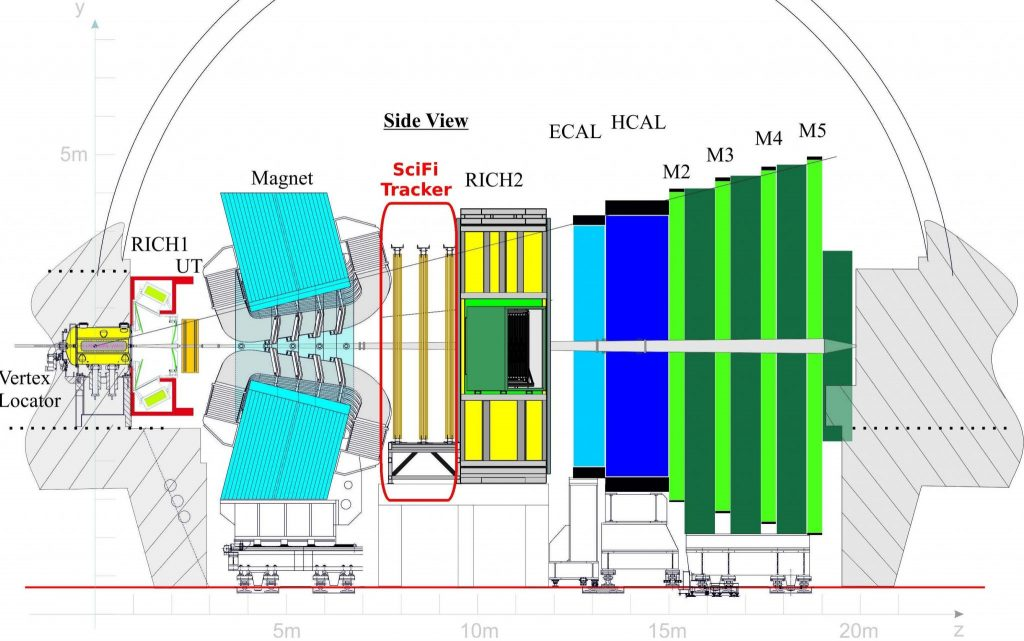
\includegraphics[width=\textwidth]{gfx/documentation/LHCb_scifi.jpeg}
        \caption{}
    \end{subfigure}
    \hfill
    \begin{subfigure}{0.48\textwidth}
        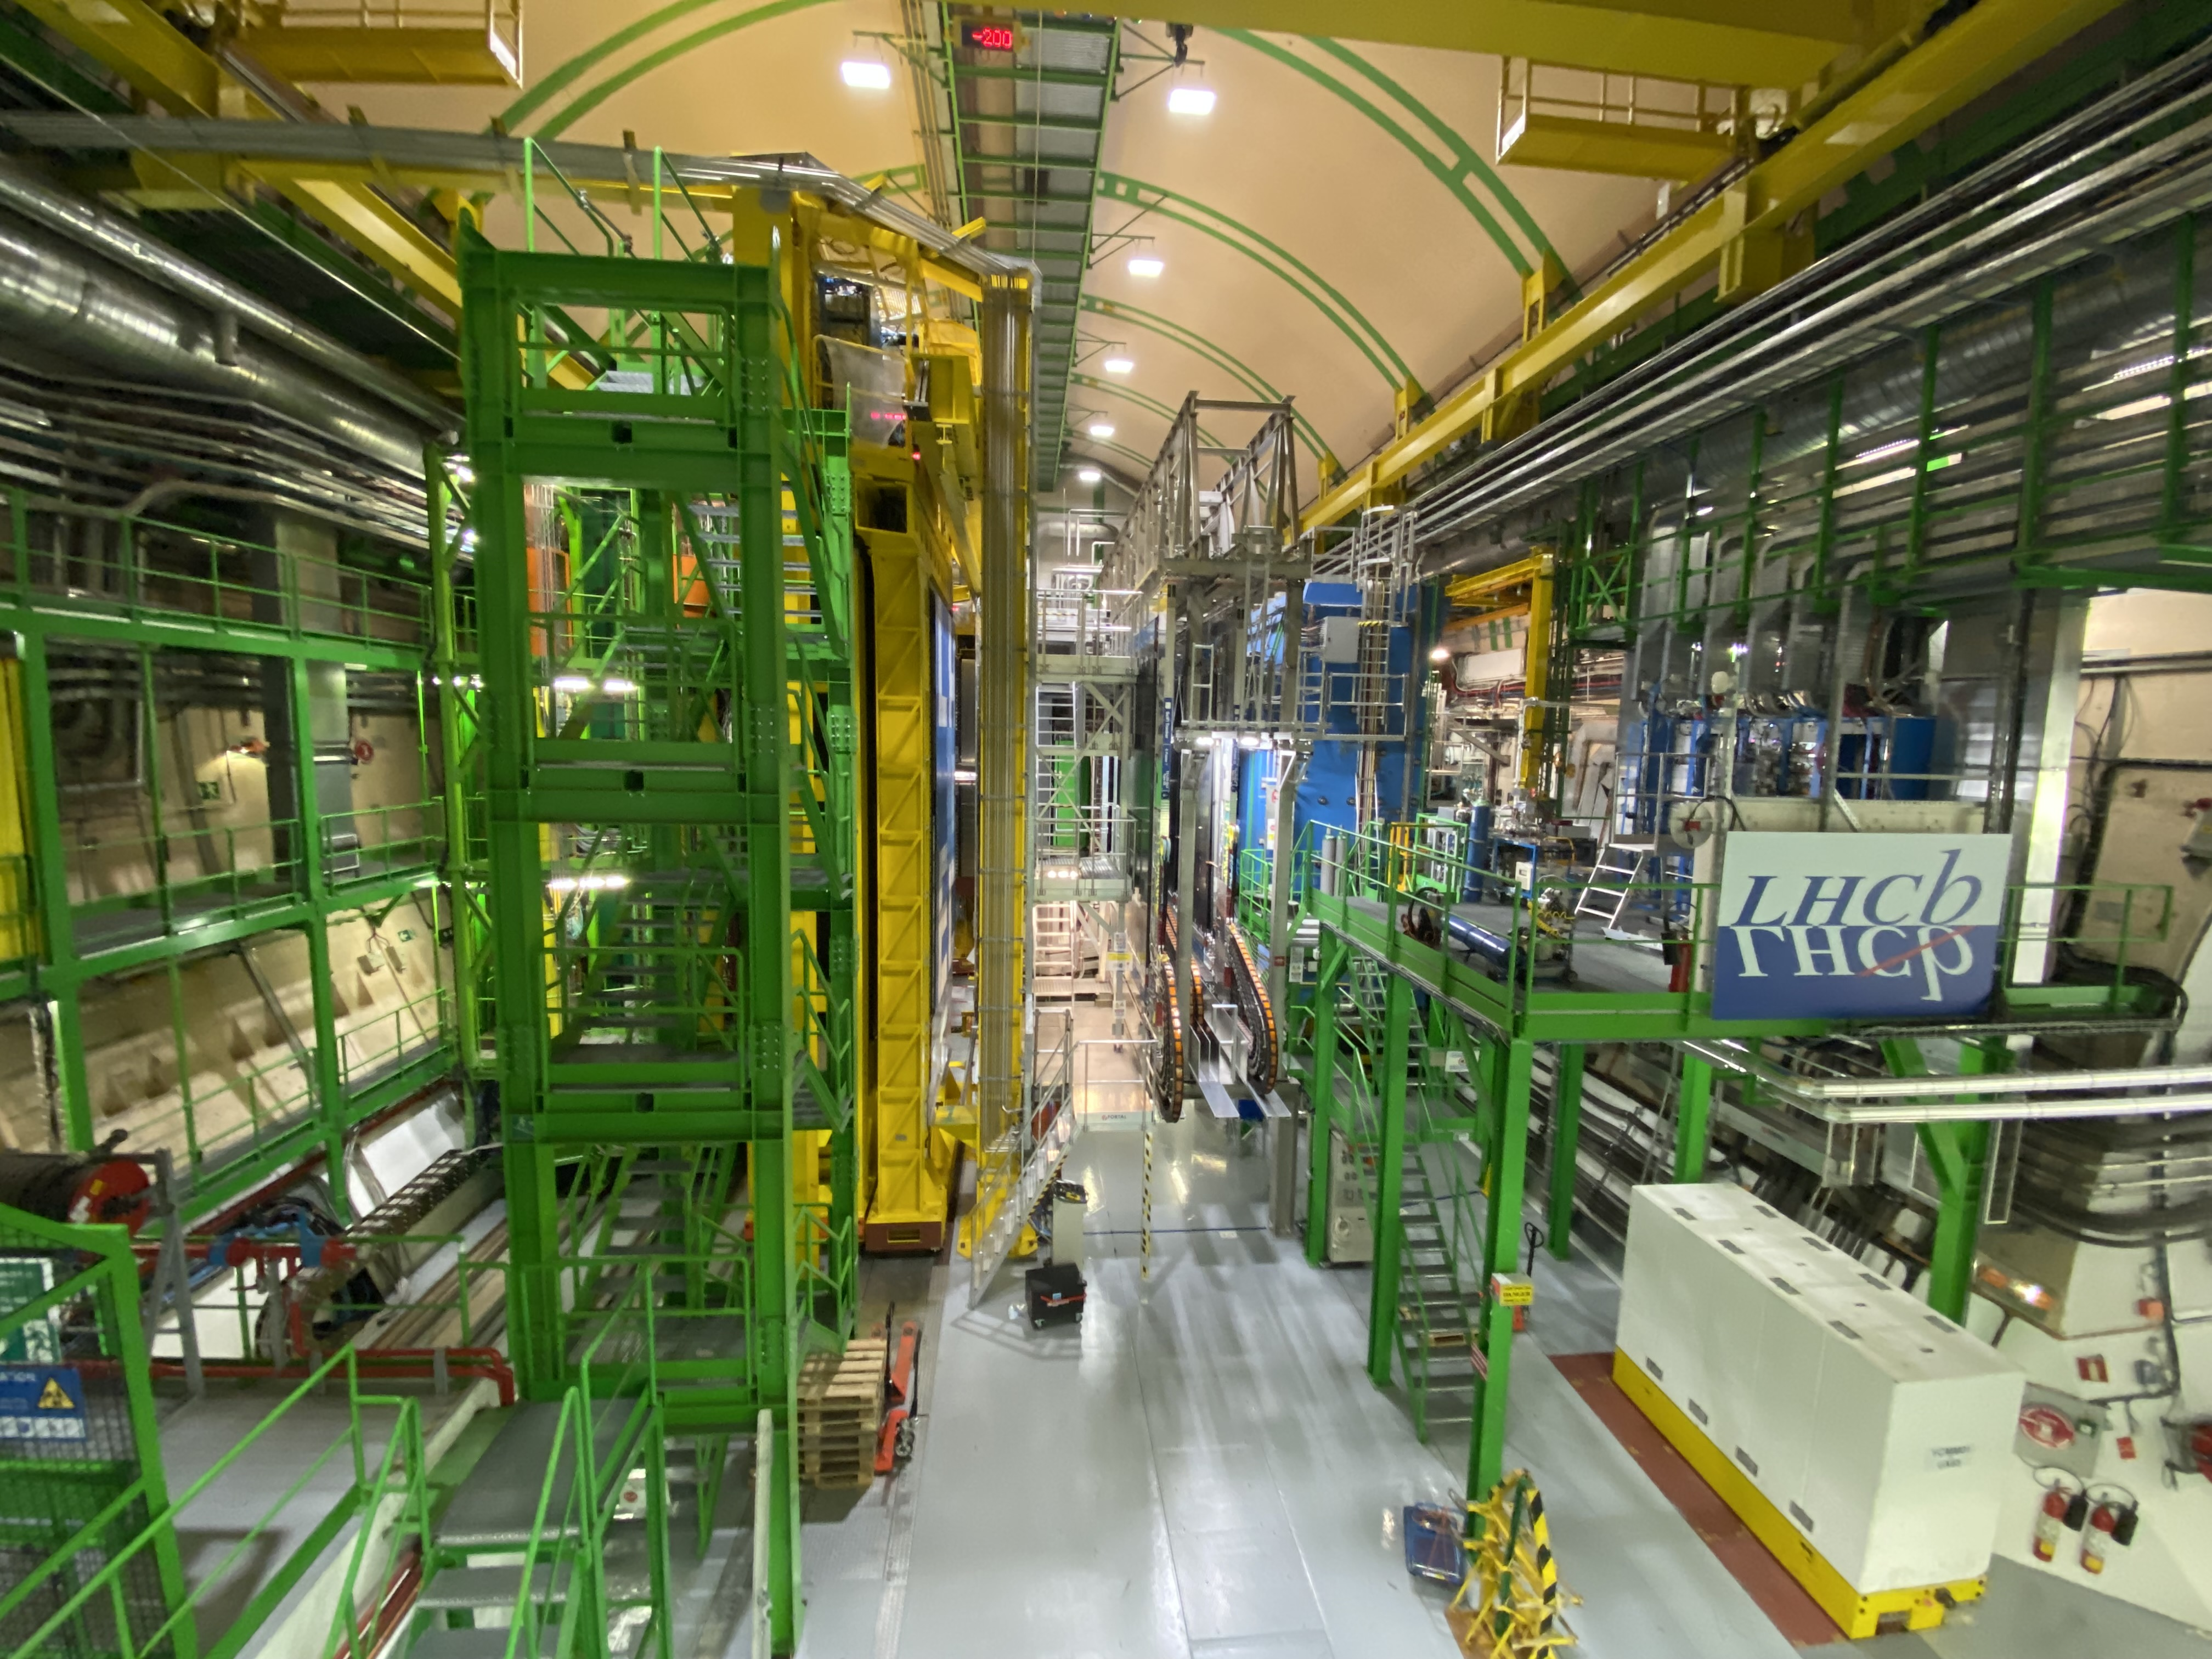
\includegraphics[width=\textwidth]{gfx/documentation/IMG_0942.jpeg}
        \caption{}
    \end{subfigure}
    \caption{LHCb detector complex with the SciFi tracker encircled in red \cite{TheEPFL} (a) and photograph of LHCb (b).}
    \label{fig:LHCb detector scheme +scifi}
\end{figure}
LHCb is made of several subdetectors, among them, the SciFi tracker made of 3 stations covering a total area of $340$ m$^2$ (see Fig. \ref{fig:scifitracker scheme}).
\begin{figure}[htbp]
    \centering
    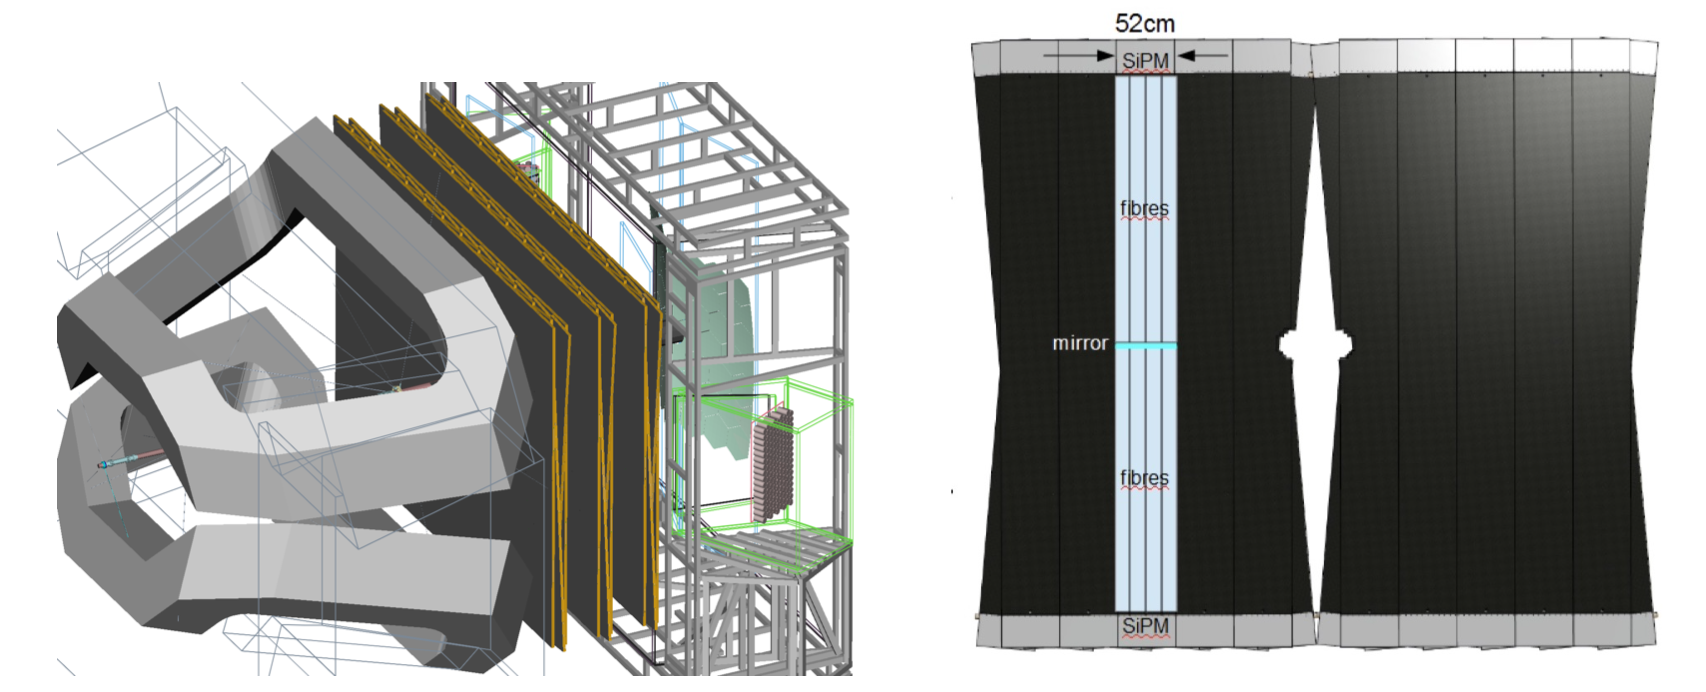
\includegraphics[width=\textwidth]{gfx/pictures/scifitracker.png}
    \caption{SciFi tracker scheme from \cite{TripplDevelopmentLHCb}.}
    \label{fig:scifitracker scheme}
\end{figure}
Each station is made of four planes oriented in different direction to obtain a spatial resolution up to \SI{100}{\micro m}. The planes are made of scintillating fibre mats. These fibres have a \SI{250}{\micro m} diameter and emit light from \SI{400}{\nano m} to \SI{600}{\nano m} with an emission peak at \SI{450}{\nano m}. SiPM arrays of \SI{250}{\micro m} summing up to $524$k channels  read out the light coming from the fibre mats. A cooling system allows to operate the SiPMs  at \SI{-40}{\celsius} in order to lower the noise due to intense radiations coming from LHC collisions. A detailed scheme shows the connection between the fibres and the SiPM in Fig. \ref{fig:fibre to sipm}.

\begin{figure}[htbp]
    \centering
    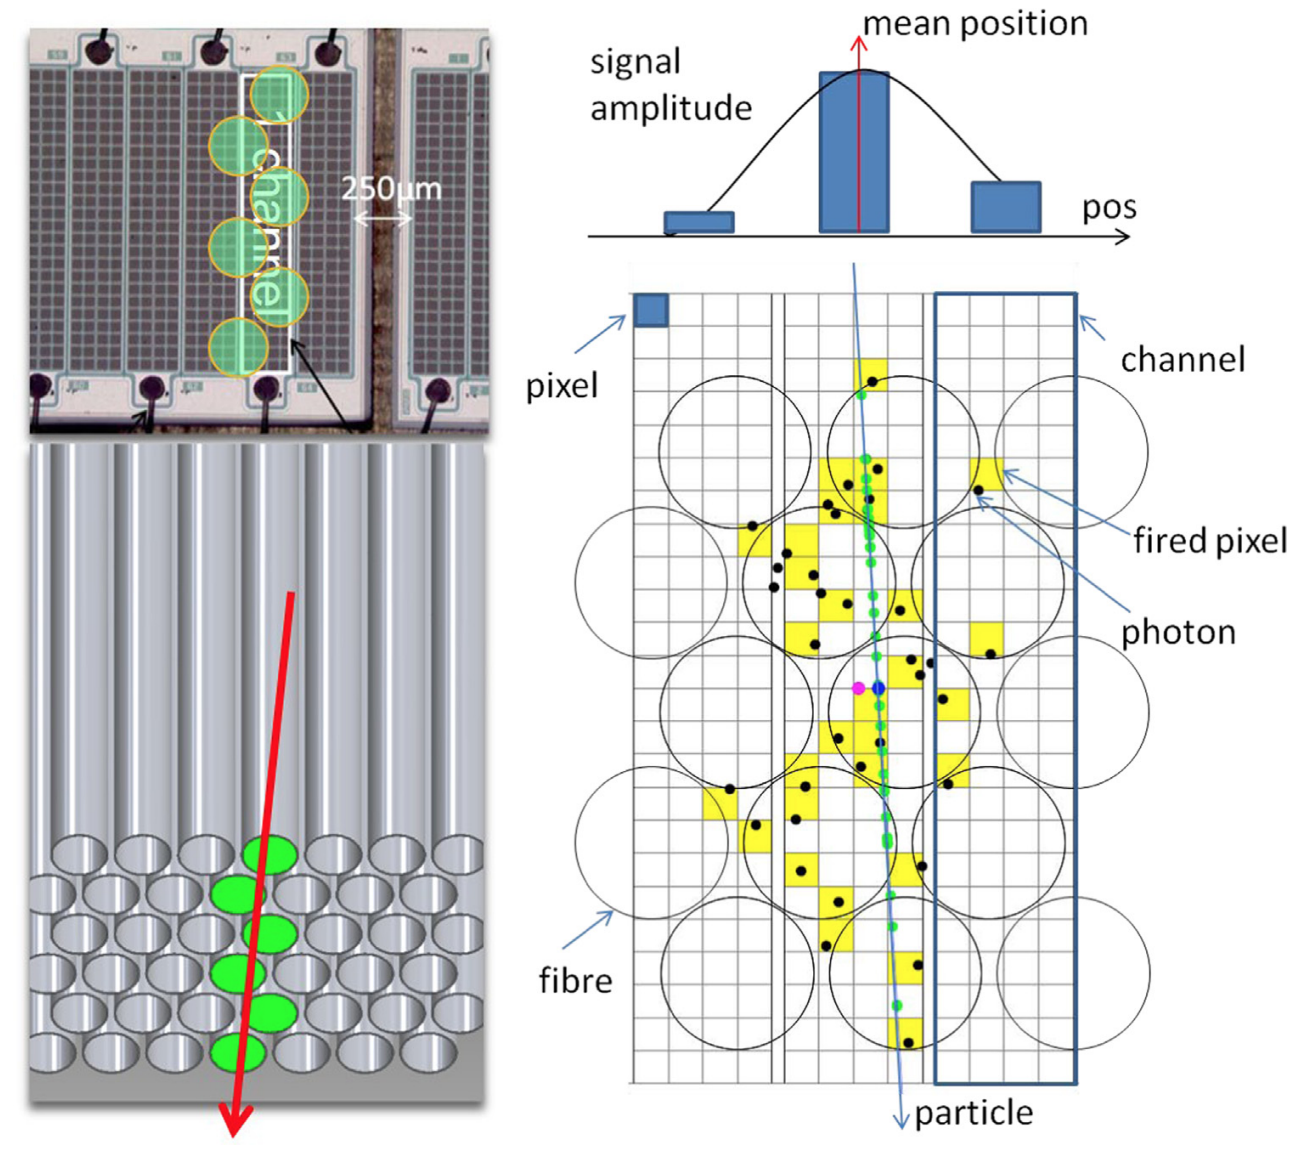
\includegraphics[width=0.9\textwidth]{gfx/pictures/fibretosipm.png}
    \caption{Scheme of the principle of the SciFi tracker. A particle hit creates photons within the fibre that are guided to the SiPM. The yellow squares represents the fired pixels the the SiPM. One can notice that there is not a one-to-one relation between a fibre and a channel (or pixel). \cite{KirnSciFi-ALHCb}.}
    \label{fig:fibre to sipm}
\end{figure}
Over time, and especially for the next LHC upgrade, where the luminosity will be increased, radiations damage the fibre in the SciFi, resulting in less light coming to the SiPMs. One way of countering this damage is to enhance the SiPM PDE either using micro lenses\cite{TripplDevelopmentLHCb}, using other SiPMs with higher PDE or both. 
A characterisation of SiPMs manufactured by the Foundation Bruno Kessler \cite{FBKKessler} is done to be used as a baseline for further R\&D about these SiPMs for the LHCb SciFi tracker.\\ 
Throughout this semester, methods for measuring the quenching resistor, breakdown voltage, correlated noise, gain and photo-detection efficiency have been implemented and adjusted to the FBK detectors.\\
\\
This thesis will firstly go into details of the working principle of a SiPMs in chapter \ref{ch:background}, then the experimental method of each measurements will be presented in chapter \ref{ch:Experimental setup and methods} and this will be followed by the presentation of the results in chapter \ref{ch:Results}.


%LPHE is responsible for providing, developing, qualifying, and testing the Silicon Photo-Multipliers (\ac{SiPM}) employed in the SciFi tracker. \ac{SiPMs} are used to readout the light emitted by the fibre mats in the tracker.\\ 
